\chapter{Simulation: Binomial Scenarios}
\section{Introduction}
This scenario models an enviroment where users have a fixed position in the space. There are some users which receive stronger signal from antenna, so they have an higher mean CQI, and others which are far from antenna and then they have smaller mean CQI. The requirements state that the distribution of CQIs must have a binomial distribution. To satisfy these, at each timeslot \(t_{j}\), every \texttt{Mobile Station} \(i\) generates a RV \(X_{i,t_{j}} \sim Bin(14,p_{i})\), and then \(CQI_{i,t_{j}} = X + 1\). By using this trick \(CQI_{i,t_{j}} \in \{1,15\}\) and it has a binomial distribution. In order to have different mean we have chose this values for parameters \(p_{i}\).
\begin{lstlisting}[caption={omnet.ini - p parameters}]
	CellularNetwork.users[0].cqi_binomial_p = 0.13
	CellularNetwork.users[1].cqi_binomial_p = 0.22
	CellularNetwork.users[2].cqi_binomial_p = 0.31
	CellularNetwork.users[3].cqi_binomial_p = 0.40
	CellularNetwork.users[4].cqi_binomial_p = 0.49
	CellularNetwork.users[5].cqi_binomial_p = 0.58
	CellularNetwork.users[6].cqi_binomial_p = 0.67
	CellularNetwork.users[7].cqi_binomial_p = 0.76
	CellularNetwork.users[8].cqi_binomial_p = 0.85
	CellularNetwork.users[9].cqi_binomial_p = 0.94
\end{lstlisting}
As in the previous scenario we will analyze the performance about throughput and response time by using both scheduler. Before doing simulation we can do some conjectures. Note that in this scenario mean CQI are sensibly different so we expect that \(user[9]\), that has highest probability to generate high CQI, and it will have highest throughput. Morover we can suppose that it will take advantage of Best CQI policy and will increase its throughput despite other users. Otherwise \(user[0]\), which has lower mean CQI, we can suppose it will decrease its throughput when it is used the Best CQI Scheduler.

\begin{itemize}
	\item \(n=10\)
	\item \(packetsize_{i} \sim U(3,75), \quad 0 \le i \le n-1\)
	\item \(CQI_{i} \sim Bin(14,p_{i})+1, \quad 0 \le i \le n-1\)
	\item \( \lambda = \lambda_{i} = 0.1 + 0.5k, \quad k\in\{1,2\ldots,19\}, \quad 0 \le i \le n-1\)
\end{itemize}

\section{Binomial, Fair Scheduler}
In this scenario the scheduler is the basic Round Robin scheduler.

\begin{figure}[H]
  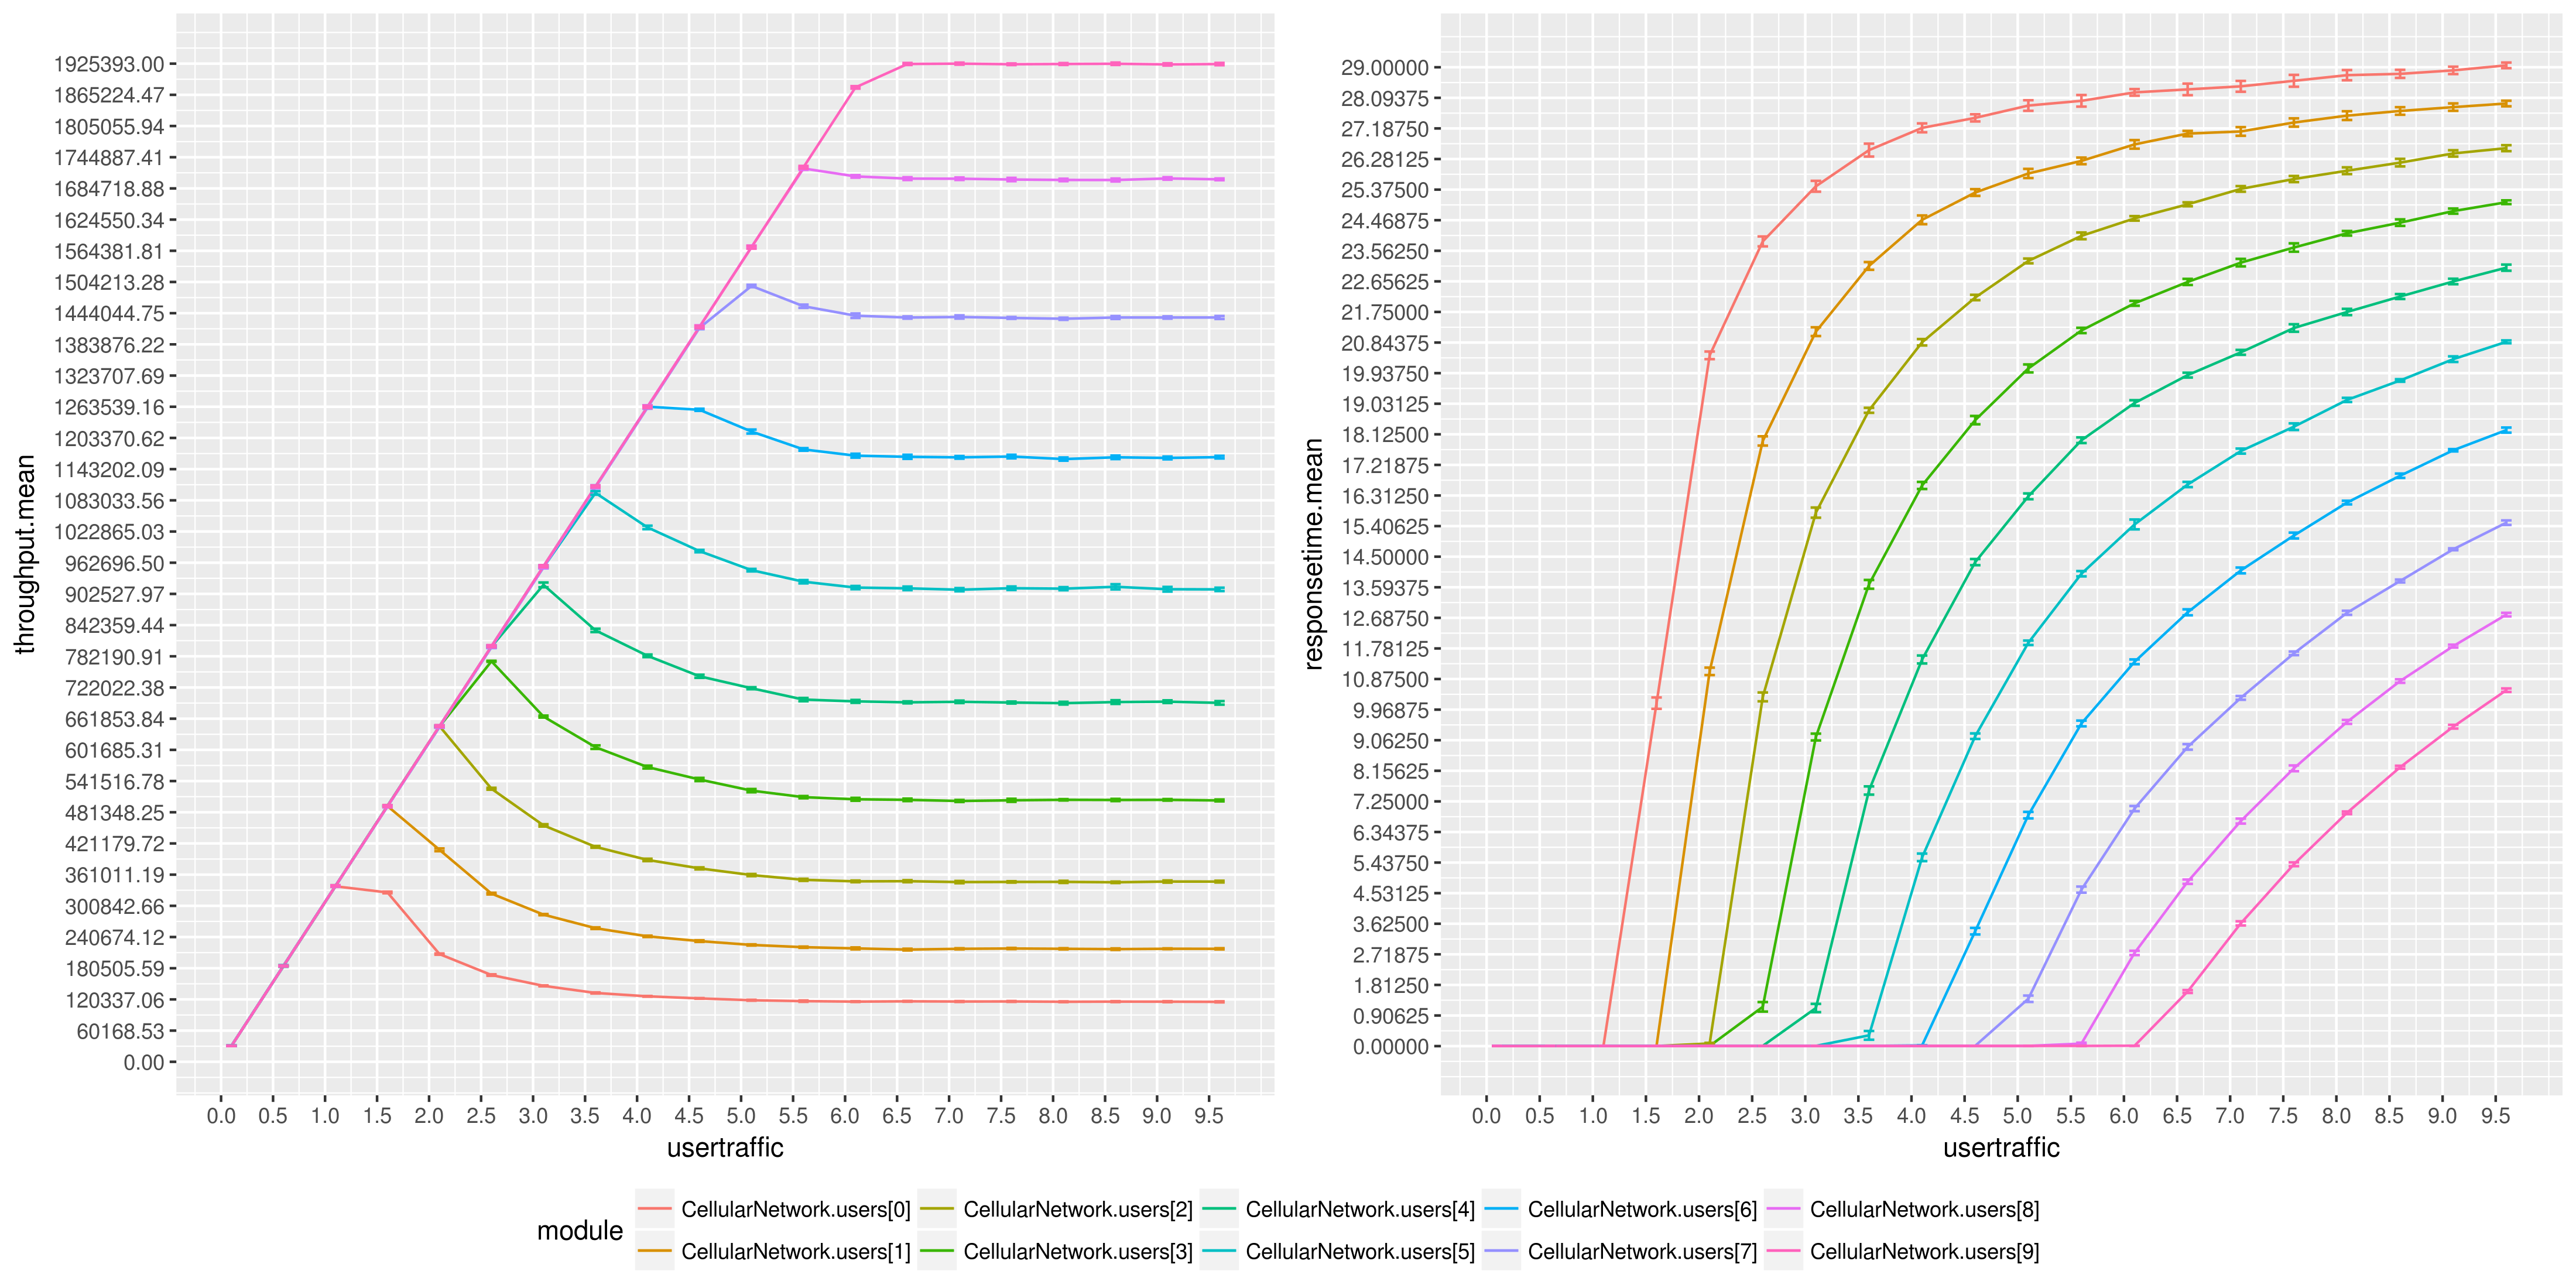
\includegraphics[width=1\textwidth]{images/binom}
  \caption{Binomial scenario - Fair: throughput, response time}
  \label{fig:Binomial scenario - Fair: throughput, response time}
\end{figure}
Users have very different throughput as we expected. When \( 0 < \lambda \leq 1\), all users have the same throughput because the traffic is very low and the resources provided by the frame are quite enough to satisfy all users. However this is a very special case, we can see that as \(\lambda\) increases users having lower mean CQIs saturate. The scheduler is always fair but users with higher mean CQIs have bigger RBs inside the frame that can carry more data. Saturation points follow the distribution of CQIs among users, so users with lower CQI, on average, saturate before, otherwise users with higher CQI exploit better the frame and saturate with higher \(\lambda\) rate.